\documentclass[acmsmall]{acmart}
\usepackage{todonotes}

\setcopyright{acmlicensed}
\copyrightyear{2018}
\acmYear{2018}
\acmDOI{XXXXXXX.XXXXXXX}

\acmJournal{TOMS}
\acmVolume{37}
\acmNumber{4}
\acmArticle{111}
\acmMonth{8}

\usepackage{listings}
\usepackage{siunitx}

\definecolor{diffincl}{RGB}{0,128,0}
\definecolor{diffrem}{RGB}{255,69,0}

\lstdefinelanguage{diff}{
  basicstyle=\ttfamily\small,
  morecomment=[f][\color{diffincl}]{+\ },
  morecomment=[f][\color{diffrem}]{-\ },
}

\newcommand{\jake}[1]{\todo[inline, backgroundcolor=green!20!white]{Jake:~#1}}


\begin{document}

\title{TBC}

\author{TBC}
\authornote{Both authors contributed equally to this research.}
\email{TBC@TBC.com}
\orcid{TBC}
\author{TBC}
\correspondingauthor
\authornotemark[1]
\email{TBC@TBC.com}
\affiliation{%
  \institution{TBC}
  \city{TBC}
  \state{TBC}
  \country{TBC}
}

\renewcommand{\shortauthors}{TBC et al.}

\begin{abstract}
  A clear and well-documented \LaTeX\ document is presented as an
  article formatted for publication by ACM in a conference proceedings
  or journal publication. Based on the ``acmart'' document class, this
  article presents and explains many of the common variations, as well
  as many of the formatting elements an author may use in the
  preparation of the documentation of their work.
\end{abstract}

%% The code below is generated by the tool at http://dl.acm.org/ccs.cfm.
\begin{CCSXML}
<ccs2012>
   <concept>
       <concept_id>10002950.10003705</concept_id>
       <concept_desc>Mathematics of computing~Mathematical software</concept_desc>
       <concept_significance>500</concept_significance>
       </concept>
   <concept>
       <concept_id>10011007.10011006.10011072</concept_id>
       <concept_desc>Software and its engineering~Software libraries and repositories</concept_desc>
       <concept_significance>300</concept_significance>
       </concept>
   <concept>
       <concept_id>10010405.10010432</concept_id>
       <concept_desc>Applied computing~Physical sciences and engineering</concept_desc>
       <concept_significance>100</concept_significance>
       </concept>
   <concept>
       <concept_id>10010405.10010444</concept_id>
       <concept_desc>Applied computing~Life and medical sciences</concept_desc>
       <concept_significance>100</concept_significance>
       </concept>
 </ccs2012>
\end{CCSXML}

\ccsdesc[500]{Mathematics of computing~Mathematical software}
\ccsdesc[300]{Software and its engineering~Software libraries and repositories}
\ccsdesc[100]{Applied computing~Physical sciences and engineering}
\ccsdesc[100]{Applied computing~Life and medical sciences}

\keywords{Scientific computing, Python, GPU computing}

\received{20 February 2007}
\received[revised]{12 March 2009}
\received[accepted]{5 June 2009}

\maketitle


\section{Introduction}

\section{Support for Graphics Processing Units (GPUs) and Just-in-Time (JIT) Compilation
Through the Python Array API Standard}

Thanks to NumPy's success~\cite{Harris2020} in unifying the two early array libraries for
Python, Numeric~\cite{Dubois1996,ascher2000numerical} and
numarray~\cite{Greenfield2003numarrayA}, SciPy's functionality, for most of its
existence, has been built on top of NumPy arrays. However, driven in part
by the boom in machine learning and artificial intelligence, graphics
processing units (GPUs) have become an
important tool for scientific computing. At the same time, advanced compiler and
program-transformation techniques, such as just-in-time (JIT) compilation
and automatic differentiation, are becoming increasingly common in computational
workflows. This posed a
problem for SciPy because, while NumPy has been the de
facto standard for array computing in Python, it does not natively support GPU computing, JIT
compilation, or automatic differentiation. This has led to the proliferation of other
array libraries for Python, such as CuPy~\cite{cupy_learningsys2017},
JAX~\cite{jax2018github}, and PyTorch~\cite{Ansel2024}, which provide support for these
capabilities (among other features). This has
effectively led to a dichotomy: SciPy cannot utilize the new features offered by these
libraries, and these new array libraries cannot make full use of the large amount of
functionality SciPy provides. Furthermore, as SciPy provides the foundational methods
for many other scientific Python packages, this also prevents these packages from
taking advantage of these developments.

Addressing this fragmentation through the Python array API standard~\cite{Meurer2023} has been a
major focus of SciPy 2.0. This standard defines application
programming interfaces (APIs) and behaviours for arrays and their
associated operations. Most importantly for SciPy, this enables
``array-consuming libraries to accept and operate on arrays from multiple different
array libraries''~\cite{Meurer2023}. In doing so, this also enables libraries that are
heavily reliant on SciPy, such as scikit-learn~\cite{scikit-learn,sklearn_api}, to
begin adopting the Python array API standard themselves.

In principle, by rewriting SciPy's functionality
in terms of these standardised APIs, SciPy can support any array package that
implements the standard. However, in practice, there are a number of barriers to this
interoperable ideal.
Most significantly, NumPy, CuPy, JAX, and PyTorch all predate
the creation of the standard\footnote{The first version of the Python array API
standard was released in December 2021, with new revisions appearing annually.}
and are therefore not fully compliant with it. To resolve this, the array-api-compat package provides lightweight wrappers that adapt these libraries' interface to the standard. Likewise,
some functionality is not covered by the standard, for a variety of reasons, so the
array-api-extra package provides generic implementations of these operations.
These additional packages therefore overcome many of the practical difficulties in
achieving interoperability. As an example, Listing~\ref{lst:fiedler} shows how a typical
function from SciPy, written in Python, can be adapted to accept arrays conforming to
the standard.

\begin{lstlisting}[language=diff,caption={Example showing the changes made to
  \texttt{scipy.linalg.fiedler} in order to support the Python array API standard.
  Changes include registering the function with an automated documentation and testing
  system that generates array type compatibility tables and test skips, using
  the namespace of the array type (denoted \texttt{xp}) rather than NumPy, and
  using array-api-compat and array-api-extra functionality when required.},
  label={lst:fiedler}]

+ @xp_capabilities()  # Register with documentation and testing framework
  def fiedler(a):
+     xp = array_namespace(a)  # get the namespace of the input array
-     a = np.atleast_1d(a)
+     a = xpx.atleast_nd(xp.asarray(a), ndim=1)  # from array-api-extra

-     if a.size == 0:
+     if xp_size(a) == 0:  # from array-api-compat
-         return np.array([], dtype=float)
+         return xp.empty((0, 0), dtype=xp.float64)
-     elif a.size == 1:
+     elif xp_size(a) == 1:
-         return np.array([[0.]])
+         return xp.asarray([[0.]])
      else:
-         return np.abs(a[..., :, None] - a[..., None, :])
+         return xp.abs(a[..., :, xp.newaxis] - a[..., xp.newaxis, :])
\end{lstlisting}

While the recipe shown in Listing~\ref{lst:fiedler} can be applied to most of SciPy's
Python code, a significant amount of SciPy's functionality is implemented in compiled
languages, such as Cython and C/C++.
This is typically the case when a Python implementation would not provide
satisfactory performance, for example, when an algorithm cannot be efficiently expressed
in terms of vectorised array operations, which would otherwise allow much of the
computation to be delegated to NumPy's optimised compiled code. This presents
a challenge because these functions cannot be converted to accept other array libraries
by simply rewriting them in terms of standardised array operations. SciPy has adopted three approaches to address this challenge.

The simplest approach is to convert arrays stored on the CPU to NumPy arrays using the
Python buffer protocol, perform the computation, and then convert the result back to the
original array type. While this provides a straightforward means of achieving
interoperability, it does not support JIT compilation or automatic differentiation.
Moreover, it is not a viable approach for arrays stored on the GPU because of the
significant overhead of transferring data between the CPU and GPU.

The second approach exploits the fact that array libraries such as JAX and CuPy have
already reimplemented a subset of SciPy's functionality, allowing us to \emph{delegate}
to their implementations. For functionality implemented in Python, we likewise delegate
to the array library's implementation where available, assuming that a library-specific
implementation will provide better performance than a generic implementation.

The final approach is to maintain two code paths: the original compiled code path for
NumPy arrays and a new Python code path written in terms of standardised operations.
While this allows SciPy to support alternative array libraries, it comes at the cost of code
duplication and an increased maintenance burden. Consequently, this approach is used
sparingly, in situations where maintaining two code paths provides a significant
performance benefit. For example, when executed on a GPU, a Python implementation can
outperform a compiled implementation executed on the CPU --- see
Figure~\ref{fig:benchmarks}(c).

Across all three approaches, there are a number of design principles that SciPy has
adopted in order to manage potential complications associated with accepting multiple
array types. First, the input array type and device on which the array is located is
preserved. Second, users cannot mix array types or arrays located on different
devices. Third, SciPy must not silently transfer arrays between devices (e.g.\ between
the CPU and GPU) because, as discussed above, this can incur a significant performance
penalty. Instead, any device transfers (e.g.\ to ensure all arrays are on the same
device) must be explicitly performed by the user. These principles help to avoid
unexpected performance issues and scenarios where it is ambiguous what the correct
behaviour should be.

\begin{figure}
    \centering
    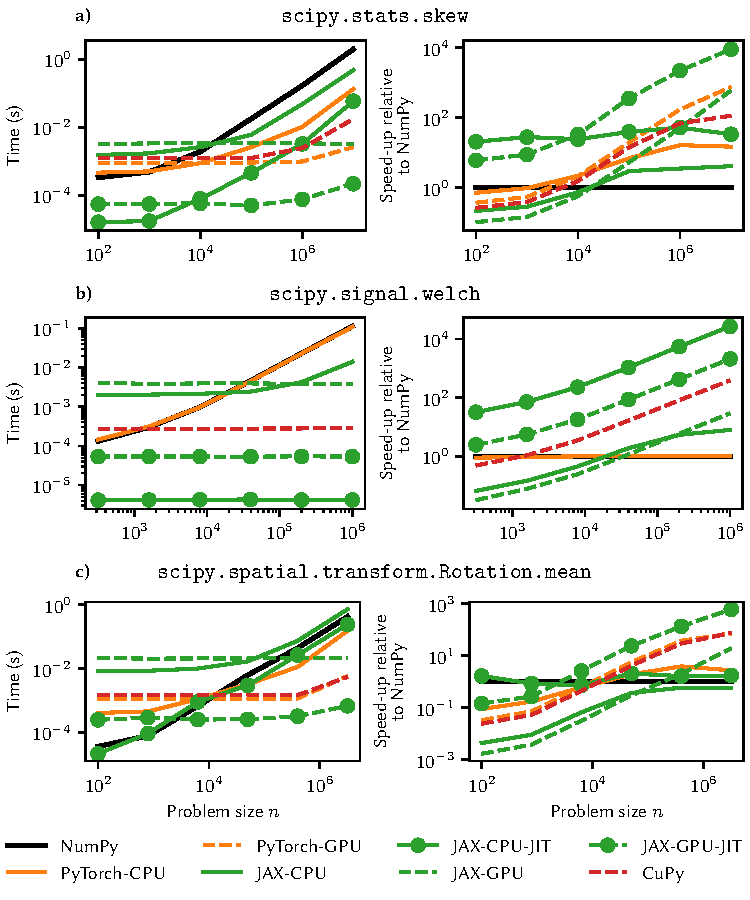
\includegraphics{figures/benchmark.pdf}
    \caption{Benchmarks comparing the performance of various SciPy functions
    for different array types as the problem size is increased. Reported
    timings are the minimum of five samples of 100 evaluations and are shown both
    as wall-clock time and relative to NumPy, with values greater than one
    indicating improved performance over NumPy.
    (a) Computing the skewness of a data set.
    (b) Estimating the power spectral density using Welch's method.
    (c) Computing the mean of multiple rotations.}\label{fig:benchmarks}
\end{figure}

While enabling users to use SciPy with their preferred array types is valuable in its
own right, it can also provide substantial performance benefits. We quantify these
benefits through a series of benchmarks covering the different approaches to adopting
the Array API Standard discussed above. All benchmarks
were executed on an Intel\textsuperscript{\textregistered}
Xeon\textsuperscript{\textregistered} Platinum 8468V Processor and
an NVIDIA H100 GPU. Code to reproduce the benchmarks is available at
\href{https://github.com/scipy/scipy-articles}{github.com/scipy/scipy-articles}.
Additional benchmarks are also presented in~\cite{Meurer2023,rotaion,rbf_bench}.

The first benchmark considers the computation of the sample skewness,
$\gamma_1 = \mu_3/\mu_2^{3/2}$, where $\mu_i$ is the biased $i$th central sample
moment, using \texttt{scipy.stats.skew}. This function is implemented entirely
in Python and was therefore adapted to accept arrays from other array libraries by
rewriting it in terms of standardised functions, similar to the example in
Listing~\ref{lst:fiedler}. Specifically, the benchmark considers computing the
skewness of three samples of size $n$, drawn from the gamma distribution (with shape
and scale parameters 5 and 0.5), the standard normal distribution, and the beta
distribution (with shape parameters 0.5 and 0.5). The computation is performed in
a vectorised fashion, with only one call to \texttt{scipy.stats.skew}.

The second benchmark considers estimating the power spectral density of a signal using
Welch's method~\cite{Welch1967} with \texttt{scipy.signal.welch}. For JAX and CuPy, this
function is delegated to their native implementations; for other array types, the input
array is converted to a NumPy array, the computation is performed, and the result is
converted back to the original array type. Consequently, PyTorch GPU results are not
included. The test signal consists of a \SI{2}{\volt_{\mathrm{RMS}}} sine wave at
\SI{1234}{\hertz}, corrupted by additive white Gaussian noise with a one-sided power
spectral density of \SI{0.001}{\volt\squared\per\hertz}, sampled at \SI{10}{\kilo\hertz}
for $n$ data points. This benchmark was also considered in~\cite{Meurer2023}; however,
here we present the results in more detail.

Finally, the third benchmark considers a series of operations involving rotations using
\path{scipy.spatial.transform.Rotation}. This is an example of functionality for which
SciPy maintains two code paths: a compiled Cython code path for NumPy arrays and a
Python code path written in terms of standardised APIs for other array types. The aim is
to maintain satisfactory performance for NumPy arrays while also supporting other array
types. The benchmark considers converting a series of $n$ random rotations, represented
as Euler angles, to quaternions, computing the chordal $L_2$ mean~\cite{Hartley2013} of
the rotations, and then converting the resulting mean back to Euler angles.

The result of these benchmarks is shown in Figure~\ref{fig:benchmarks}. In general,
these results show that for large problem sizes, using alternative array types can
provide significant performance benefits over NumPy. For small problem sizes, we see
that, with the exception JAX-JIT, the NumPy is still typically fastest option due
to the lower overhead of using NumPy arrays. However, for large problem sizes, other
array types are favoured. The benchmarks also highlight the different performance
characteristics of the approaches for handling compiled code discussed above.
For example, in the Welch's method benchmark, we see that using PyTorch arrays offers
no performance benefit as the implementation is based on converting the input array to a
NumPy array, performing the computation, and then converting the result back to a
PyTorch array. Likewise, in the rotation benchmark, we see that NumPy is very
competitive for small problem sizes due to the fact it uses a compiled code path while
other array types use a Python code path.

\begin{table}
  \caption{Coverage of modules in SciPy 2.0 supporting alternative array types.
  \jake{Update once SciPy 2.0 is released}}\label{tab:coverage}
  \begin{tabular}{lcccccc}
    \toprule
    Module & CuPy & \multicolumn{2}{c}{PyTorch} & \multicolumn{3}{c}{JAX}\\
    \cmidrule(lr){2-2}
    \cmidrule(lr){3-4}
    \cmidrule(lr){5-7}
    & GPU & CPU & GPU & CPU & GPU & JIT\\
    \midrule
\texttt{cluster} & 26 \% & 91 \% & 26 \% & 91 \% & 26 \% & 69 \% \\
\texttt{constants} & 100 \% & 100 \% & 100 \% & 100 \% & 100 \% & 100 \% \\
\texttt{differentiate} & 100 \% & 100 \% & 100 \% & 100 \% & 100 \% & 0 \% \\
\texttt{fft} & 75 \% & 100 \% & 75 \% & 94 \% & 75 \% & 94 \% \\
\texttt{integrate} & 33 \% & 30 \% & 30 \% & 27 \% & 27 \% & 17 \% \\
\texttt{interpolate} & 30 \% & 53 \% & 3 \% & 53 \% & 3 \% & 3 \% \\
\texttt{linalg} & 4 \% & 4 \% & 4 \% & 4 \% & 4 \% & 2 \% \\
\texttt{ndimage} & 92 \% & 99 \% & 0 \% & 99 \% & 1 \% & 1 \% \\
\texttt{optimize} & 12 \% & 11 \% & 11 \% & 5 \% & 5 \% & 5 \% \\
\texttt{signal} & 70 \% & 67 \% & 42 \% & 67 \% & 33 \% & 33 \% \\
\texttt{sparse} & 2 \% & 2 \% & 2 \% & 2 \% & 2 \% & 2 \% \\
\texttt{spatial} & 7 \% & 7 \% & 7 \% & 7 \% & 7 \% & 7 \% \\
\texttt{special} & 27 \% & 28 \% & 11 \% & 28 \% & 12 \% & 28 \% \\
\texttt{stats} & 43 \% & 51 \% & 37 \% & 49 \% & 41 \% & 43 \% \\
\midrule
Overall & 35 \% & 40 \% & 20 \% & 39 \% & 19 \% & 25 \% \\
  \bottomrule
\end{tabular}
\end{table}

Converting SciPy's extensive range of functionality to support alternative array types
has been a significant undertaking. Table~\ref{tab:coverage} shows the progress towards
this goal as of SciPy 2.0. \jake{Finish this once SciPy 2.0 is actually released, as it
is difficult to comment on coverage when we do not yet know what it will be.} Note that
this table omits legacy modules and modules that are not within the scope of the
conversion. This includes \texttt{scipy.datasets} and \texttt{scipy.io}, both of which
involve reading binary files that must first be loaded into CPU memory; we therefore
defer conversion to the user's preferred array type.

Future versions of SciPy will continue to expand the number of functions supporting
alternative array types as well as adding support for additional features, such as
PyTorch's JIT compilation mechanism \texttt{torch.compile}.

\section{A New Look at Language Choices}

As discussed in~\cite{Virtanen2020}, much of SciPy's original success can be attributed
to the convenient Python interfaces it provided to popular compiled numerical libraries
that were otherwise distributed primarily as standalone Fortran source
packages, such as those available through the Netlib repository~\cite{netlib}.
These included
ODEPACK~\cite{Hindmarsh1983ODEPACK},
VODE/ZVODE~\cite{Brown1989}, and DOPRI5~\cite{Hairer1987} for solving initial value
problems; QUADPACK~\cite{Piessens1983} for quadrature; FITPACK~\cite{dierckx1995curve}
for spline fitting; ID~\cite{martinsson2008id,Halko2011} for interpolative
matrix decomposition; ODRPACK~\cite{Boggs1989}
for orthogonal distance regression; COBYLA~\cite{Powell1994}, L-BFGS-B~\cite{Morales2011},
SLSQP~\cite{Kraft1994,Kraft1988SQP}, MINPACK~\cite{More1980}, and
NNLS~\cite{Lawson1995} for optimization;
ARPACK-NG~\cite{Lehoucq2023ARPACKNG} and PROPACK~\cite{Larsen1998} for sparse eigenvalue problems
and singular value decompositions, respectively; AMOS~\cite{Amos1986} and
SPECFUN~\cite{Zhang1996} for special functions;
CDFLIB~\cite{Brown1994CDFLIB}, mvndist~\cite{Genz1992}, and
statlib~\cite{Dinneen1976,Best1975,Royston1995,Maclaren1985} for probability
distributions and statistical functions;
and FFTPACK~\cite{Swarztrauber1982} for fast Fourier transforms.
Consequently, SciPy 1.0 consisted of approximately $25\%$ Fortran,
second only to Python ($50\%$)~\cite{Virtanen2020}.

Despite the enormous utility these codes have provided, they also presented a number
of challenges on the road to SciPy 2.0. By far the most significant of these was
limited availability of Fortran compilers for Windows and
emerging new platforms such as WebAssembly~\cite{Haas2017}. This left SciPy
in a precarious position where distributing SciPy was challenging and required
a custom MinGW toolchain to build SciPy on Windows~\cite{obermeier2023eu}.
While tools such as \texttt{flang-new} (now \texttt{flang})
and \texttt{LFortran} showed promise in addressing this issue, they were not
mature enough to be adopted by SciPy at the time and waiting for them to mature was
deemed not viable.

In addition, there were a number of further issues pertaining to the Fortran 77
implementations of these codes. A number of them were not thread-safe,
meaning that they could not be safely called from multiple threads simultaneously.
Previously, SciPy used locking to prevent this. However, the introduction of
free-threading in CPython 3.13, and its subsequent maturation in CPython 3.14, meant
that, for the first time, multiple threads could execute Python code concurrently
without the Global Interpreter Lock (GIL)~\cite{gross2023pep703}. Unfortunately,
users of these non-reentrant codes would not be able to take advantage of this
new feature.
Other challenges presented by these codes included a lack of support for
64-bit integer types (ILP64) and lack of control over the random number generator used.
Finally, many of these codes were no longer actively maintained, meaning that the
SciPy developers were effectively responsible for fixing any bugs that arose.
This increased the maintenance burden and made it more difficult to resolve bugs and
improve these routines. This was further compounded by a lack of expertise in Fortran
77 within the SciPy developer community, which often led to bugs remaining unresolved
indefinitely.

\begin{figure}
    \centering
    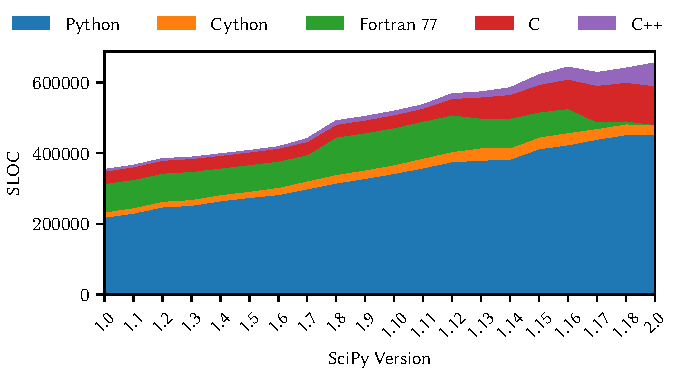
\includegraphics{figures/sloc.pdf}
    \caption{Source lines of code (SLOC) in SciPy by programming language.
    Libraries that are wrapped by SciPy and are actively maintained projects themselves,
    e.g.\ Boost.\@Math~\cite{boostmath} and HiGHS~\cite{Huangfu2017}, are excluded.
    For the SLOC including these libraries see Figure~\ref{fig:sloc_all} in
    Appendix~\ref{sec:appendix_sloc}.}\label{fig:sloc}
\end{figure}

After careful evaluation of the above issues, it was decided that these
codes needed either to be replaced with
more recent, actively maintained alternatives, or to be translated from their
original Fortran 77 source code to either pure Python,
Cython~\cite{Behnel2011}, or C/C++ in order to secure the long-term future of the
project. Consequently, COBYLA has been replaced with
a Python implementation from the PRIMA~\cite{Zhang_2023} package, FFTPACK has been replaced with
ducc.\@fft~\cite{reinecke2019ducc}, and some of the special and statistical functions
mentioned have been replaced with counterparts from Boost.\@Math~\cite{boostmath}. Translation of the remaining
codes posed a significant undertaking, requiring a significant proportion of SciPy's
$\sim80{,}000$ source lines of Fortran 77 to be translated by hand. The completion of this work has been a major milestone for
SciPy 2.0, leading to the resolution of the challenges described above as well as many
long-standing bugs. Furthermore, these translations provide the foundation for
future development and improvements, for example, improved special functions, as
discussed below.
\jake{Add a forward reference to the relevant section.}
Such developments were previously infeasible
due to the lack of expertise in Fortran 77 within the SciPy developer community.
Following these changes, SciPy 2.0 contains no Fortran, as illustrated by
Figure~\ref{fig:sloc}, which shows how the language composition of SciPy has changed
since version 1.0.

\section{Universal Random Variate Generation Methods}

The \texttt{stats} module in SciPy supports calculations for a large number of
probability distributions, including the generation of random variates.
These sampling algorithms are often specifically designed for a given
distribution, e.g., by relying on general methods such as inversion of the
CDF\footnote{Note that accurate and fast CDF inversion is usually non-trivial.}
or on the rejection principle~\cite{vonneumann1951}. In contrast, there are
also so-called automatic or black-box methods: the same implementation can be
used to sample from large classes of distributions, while requiring only basic
information about the distribution --- such as the density (and optionally
its derivative), the CDF, and/or the mode (see~\cite{hormann2004} for an
overview). Based on this input, a generator is automatically derived in a
setup step, which can then be used to draw random variates of the
distribution.

Although such universal methods were originally motivated by nonstandard
distributions~\cite{hormann2004}, they offer advantages that make them attractive
even for standard ones (see~\cite{derflinger2010} for further use cases):
\begin{itemize}
\item They can be used to sample from truncated distributions.
\item For inversion-based methods, the structural properties of the
underlying uniform random number generator are preserved, and numerical
accuracy can be controlled via a parameter --- making these methods
well-suited to quasi-Monte Carlo (QMC) simulations.
\item Depending on the use case, one can choose between a fast setup with
slow marginal generation time, or vice versa.
\end{itemize}

The \texttt{stats.sampling} sub-module implements several such algorithms for
continuous distributions, namely transformed density
rejection~\cite{hormann1995, gilks1992}, polynomial-~\cite{derflinger2010} or
Hermite-interpolation-based~\cite{hormann2003} CDF inversion, and the simple
ratio-of-uniforms method~\cite{leydold2001, leydold2003}, as well as for
discrete distributions, i.e., guide-table~\cite{chen1974} and
alias-urn~\cite{walker1977} methods, all built on the C library UNU.RAN~\cite{hormann2007}.
For convenience, \texttt{FastGeneratorInversion}
can be used to create a generator based on the inversion method from supported continuous
\texttt{scipy.stats} distributions. For further details and benchmarking,
please see~\cite{baumgarten2022}.

\begin{acks}
We thank everyone who has contributed to SciPy 2.0, from those who have posted one
comment about an issue through those who have made several small patches and beyond.

This work received support from the
\grantsponsor{CZI}{Chan Zuckerberg Initiative Essential Open Source Software for Science}{https://chanzuckerberg.com/eoss/}
through the grants:
\grantnum[https://chanzuckerberg.com/eoss/proposals/a-solid-foundation-for-statistics-in-python-with-scipy/]{CZI}{A Solid Foundation for Statistics in Python with SciPy},
\grantnum[https://chanzuckerberg.com/eoss/proposals/advancing-an-inclusive-culture-in-the-scientific-python-ecosystem/]{CZI}{Advancing an Inclusive Culture in the Scientific Python Ecosystem},
\grantnum[https://chanzuckerberg.com/eoss/proposals/sparse-arrays-for-scientific-python/]{CZI}{Sparse Arrays for Scientific Python},
\grantnum[https://chanzuckerberg.com/eoss/proposals/scipy-fundamental-tools-for-biomedical-research/]{CZI}{SciPy: Fundamental Tools for Biomedical Research},
and
\grantnum[https://chanzuckerberg.com/eoss/proposals/advancing-array-interoperability-within-the-pydata-ecosystem/]{CZI}{Advancing Array Interoperability Within the PyData Ecosystem};
\grantsponsor{NASA}{NASA Research Opportunities for Space and Earth Science}{https://science.nasa.gov/researchers/sara/grant-solicitations/}
through the grants:
\grantnum{NASA}{Reinforcing the Foundations of Scientific Python}
and
\grantnum{NASA}{Ensuring a Fast and Secure Core for Scientific Python – Security, Accessibility and Performance of NumPy, SciPy and scikit-learn; Going Beyond NumPy With Accelerator Support};
the
\grantsponsor{NF}{NumFOCUS Small Development Grants (SDG) program}{https://numfocus.org/programs/small-development-grants}
through the grants:
\grantnum{NF}{An Efficient, High-Level Implementation of Linear Programming},
\grantnum{NF}{Maturing a sparse array implementation for SciPy},
\grantnum{NF}{Enhanced LAPACK Support in SciPy},
\grantnum{NF}{Complete the SciPy special functions documentation},
\grantnum{NF}{SciPy Development Documentation Overhaul},
\grantnum{NF}{Improving boundary handling and data type support in scipy.ndimage},
\grantnum{NF}{A Mixed Integer Programming Solver for SciPy},
\grantnum{NF}{Add PROPACK Sparse SVD to SciPy},
\grantnum{NF}{Introducing Users to Powerful New Features of SciPy},
\grantnum{NF}{Faster Random Variate Sampling from SciPy Statistical Distributions},
and
\grantnum{NF}{Streamlined Special Function Development in SciPy};
and Tidelift for their regular donations to the project.

\end{acks}

\bibliographystyle{ACM-Reference-Format}
\bibliography{references}

\appendix
\section{Additional SLOC Plots}\label{sec:appendix_sloc}

\begin{figure}[h]
    \centering
    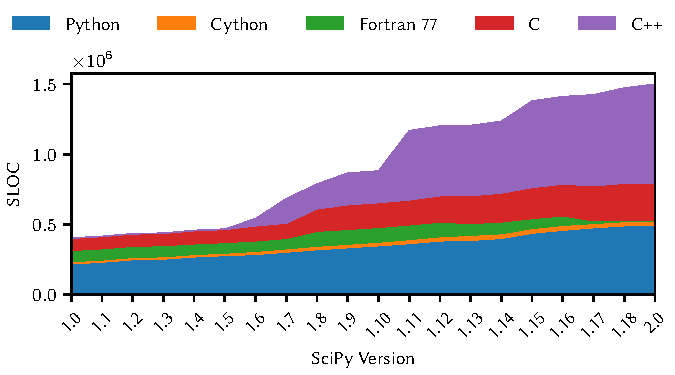
\includegraphics{figures/sloc_all.pdf}
    \caption{Source lines of code (SLOC) in SciPy by programming language, including all
    libraries that are wrapped by SciPy.}\label{fig:sloc_all}
\end{figure}
\end{document}
\endinput
